\documentclass[a4paper,12pt,twoside]{book}
\usepackage[utf8]{inputenc}
\usepackage{amsmath}
\usepackage{amsfonts}
\usepackage{xcolor}
\usepackage{tikz}
\usepackage[most]{tcolorbox}
\usepackage{amssymb}
\usepackage[left=2.00cm, right=2.00cm, top=2.00cm, bottom=2.00cm]{geometry}
\usepackage{pgfplots}
\pgfplotsset{compat=1.15}
\usepackage{hyperref}
\usetikzlibrary{arrows}


\pagestyle{empty}









\renewcommand\thesection{\arabic{section}}
\renewcommand\thesubsection{\thesection.\arabic{subsection}}
\renewcommand{\baselinestretch}{1.7}
\title{Trigonometric Ratio In Olympiad Geometry}
\author{Trinh Quoc Khanh}
\date{12 / 12 / 2022}
\setlength{\parindent}{0pt}
\pagestyle{none}

\newtcolorbox{mybox}{
	enhanced,
	boxrule=0pt,frame hidden,
	borderline west={4pt}{0pt}{black!50!black},
	colback=black!10!white,
	sharp corners
}

\newenvironment{dedication}
    {\begin{quotation}\begin{center}\begin{em}}
    {\par\end{em}\end{center}\end{quotation}}





\begin{document}

\maketitle
\tableofcontents
\newpage
\textbf{\begin{center}\large{Abstract}\end{center}}
\small{When solving olympiad geometry problems, we often need to simplify the hypothesis from complex things to easy ones, and ratio is a very useful tool to do this work. Furthermore, it can even make the given statement equivalent to something trivial (like the Law of Sines, etc.).\\
If you see a mistake in this article, please don't hesitate to contact me at \textit{\textcolor{blue}{trinhquockhanh@pm.me}}
\begin{center}
    \noindent\rule{12cm}{0.4pt}
\end{center}
\begin{dedication}
Dedicated to my family and my form teacher for their never-ending inspirations
\end{dedication}
\begin{center}
    \noindent\rule{12cm}{0.4pt}
\end{center}
\section{Theorems and properties}


\textbf{1.} Given a triangle $ABC$, with $D\in BC$, we have: $\dfrac{DB}{DC}=\dfrac{AB}{AC}.\dfrac{sin\angle{DAB}}{sin\angle{DAC}}$

\begin{center}
		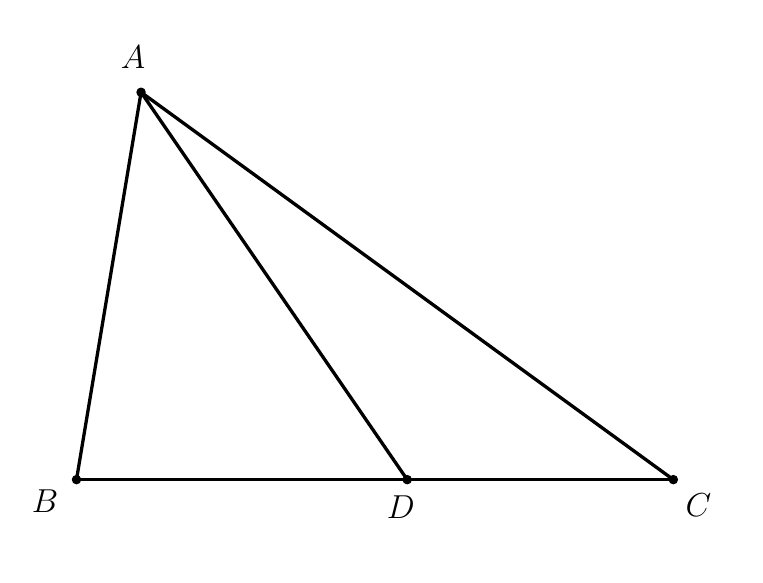
\begin{tikzpicture}[line cap=round,line join=round,>=triangle 45,x=1.0cm,y=1.0cm]
			\clip(2.24,-1.46) rectangle (11.22,5.24);
			\draw [line width=1.2pt] (3.68,4.42)-- (2.86,-0.5);
			\draw [line width=1.2pt] (2.86,-0.5)-- (10.44,-0.5);
			\draw [line width=1.2pt] (10.44,-0.5)-- (3.68,4.42);
			\draw [line width=1.2pt] (7.06,-0.5)-- (3.68,4.42);
			\begin{scriptsize}
				\draw [fill=black] (3.68,4.42) circle (1.5pt);
				\draw[color=black] (3.58,4.87) node {\large{$A$}};
				\draw [fill=black] (2.86,-0.5) circle (1.5pt);
				\draw[color=black] (2.46,-0.77) node {\large{$B$}};
				\draw [fill=black] (10.44,-0.5) circle (1.5pt);
				\draw[color=black] (10.76,-0.83) node {\large{$C$}};
				\draw [fill=black] (7.06,-0.5) circle (1.5pt);
				\draw[color=black] (6.98,-0.85) node {\large{$D$}};
			\end{scriptsize}
		\end{tikzpicture}
\end{center}
\textbf{Proof.} We have: $\dfrac{DB}{DC}=\dfrac{[ABD]}{[ACD]}=\dfrac{\dfrac{1}{2}AB.AD.sin\angle{DAB}}{\dfrac{1}{2}AC.AD.sin\angle{DAC}}=\dfrac{AB}{AC}.\dfrac{sin\angle{DAB}}{sin\angle{DAC}}$.\\\\
\textit{$-$ This is a fundamental yet crucial property if you want to utilize the ratio tool to solve a geometry problem since it links the segment lengths to the trigonometric expression of angles. If you like dealing with geometry length, think about whether there are any unique configurations, such as obtuse triangles, opposite directed segments, etc. Otherwise, your answer might not be correct.}
\newpage
To establish collinearity, we have some ideas:\\
\textbf{2.} Given a triangle $ABC$, $D\in AB$, $DE\parallel BC$, we have: $E\in AC \Leftrightarrow \dfrac{\overline{DE}}{\overline{BC}}=\dfrac{\overline{AD}}{\overline{AB}}$
\begin{center}
	\begin{tikzpicture}[line cap=round,line join=round,>=triangle 45,x=1.0cm,y=1.0cm]
		\clip(2.06,-1.44) rectangle (11.24,5.18);
		\draw [line width=1.2pt] (3.68,4.42)-- (2.86,-0.5);
		\draw [line width=1.2pt] (2.86,-0.5)-- (10.44,-0.5);
		\draw [line width=1.2pt,dash pattern=on 3pt off 3pt] (10.44,-0.5)-- (3.68,4.42);
		\draw [line width=1.2pt] (3.3070534154638227,2.182320492782936)-- (6.754535257883608,2.182320492782936);
		\begin{scriptsize}
			\draw [fill=black] (3.68,4.42) circle (1.5pt);
			\draw[color=black] (3.58,4.87) node {\large{$A$}};
			\draw [fill=black] (2.86,-0.5) circle (1.5pt);
			\draw[color=black] (2.46,-0.77) node {\large{$B$}};
			\draw [fill=black] (10.44,-0.5) circle (1.5pt);
			\draw[color=black] (10.76,-0.83) node {\large{$C$}};
			\draw [fill=black] (3.3070534154638227,2.182320492782936) circle (1.5pt);
			\draw[color=black] (2.98,2.53) node {\large{$D$}};
			\draw [fill=black] (6.754535257883608,2.182320492782936) circle (1.5pt);
			\draw[color=black] (7.02,2.61) node {\large{$E$}};
		\end{scriptsize}
	\end{tikzpicture}
\end{center}
\textbf{Hint.} Let $AE$ intersect $BC$ at $C'$. Prove that $C\equiv C'$.\\
\textit{This can be used in conjunction with the Thales theorem to prove collinearity in issues where there are a number of parallel lines, which is sometimes very helpful.}\\
\textbf{3.} \textbf{Menelaus} and \textbf{Ceva} theorem \\
$\bullet$ \textbf{Menelaus theorem}
\begin{center}
	\begin{tikzpicture}[line cap=round,line join=round,>=triangle 45,x=1.0cm,y=1.0cm]
		\clip(1.86,-1.5) rectangle (14.38,5.4);
		\draw [line width=1.2pt] (4.,4.42)-- (2.86,-0.5);
		\draw [line width=1.2pt] (2.86,-0.5)-- (10.4,-0.52);
		\draw [line width=1.2pt] (10.4,-0.52)-- (4.,4.42);
		\draw [line width=1.2pt,dash pattern=on 3pt off 3pt] (3.661324350399836,2.958347196462451)-- (13.423957783641162,-0.5280211081794195);
		\draw [line width=1.2pt] (13.423957783641162,-0.5280211081794195)-- (10.4,-0.52);
		\begin{scriptsize}
			\draw [fill=black] (4.,4.42) circle (1.5pt);
			\draw[color=black] (3.9,4.99) node {\large{$A$}};
			\draw [fill=black] (2.86,-0.5) circle (1.5pt);
			\draw[color=black] (2.36,-0.77) node {\large{$B$}};
			\draw [fill=black] (10.4,-0.52) circle (1.5pt);
			\draw[color=black] (10.6,-0.89) node {\large{$C$}};
			\draw [fill=black] (13.423957783641162,-0.5280211081794195) circle (1.5pt);
			\draw[color=black] (13.82,-0.87) node {\large{$D$}};
			\draw [fill=black] (7.815683222705425,1.4747695124742501) circle (1.5pt);
			\draw[color=black] (8.04,1.87) node {\large{$E$}};
			\draw [fill=black] (3.661324350399836,2.958347196462451) circle (1.5pt);
			\draw[color=black] (3.18,3.17) node {\large{$F$}};
		\end{scriptsize}
	\end{tikzpicture}
\end{center}	
Given a triangle $ABC$. The points $D, E, F$ lie on the lines $BC, CA, AB$, respectively. From here $D, E, F$ are collinear if and only if:$${\displaystyle {\frac {\overline {FA}}{\overline {FB}}}\cdot {\frac {\overline {DB}}{\overline {DC}}}\cdot {\frac {\overline {EC}}{\overline {EA}}}=1}$$
\newpage
$\bullet$ \textbf{Ceva theorem}
\begin{center}
	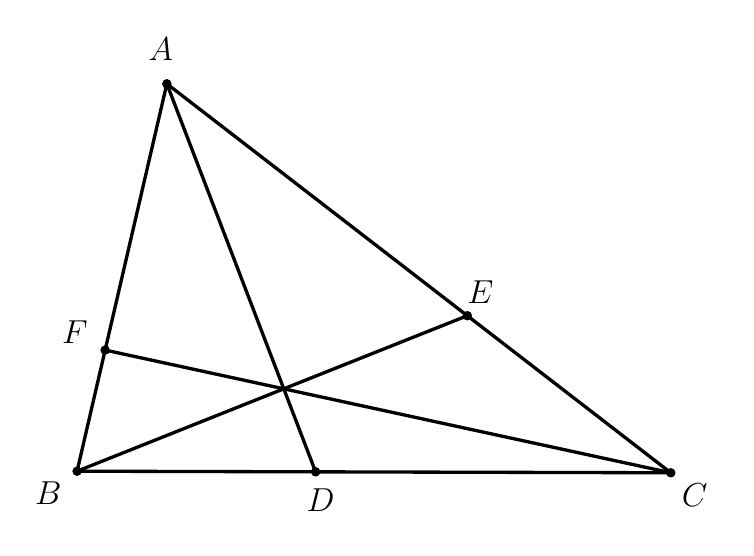
\begin{tikzpicture}[line cap=round,line join=round,>=triangle 45,x=1.0cm,y=1.0cm]
		\clip(2.2326553133118168,-1.2163260197690284) rectangle (11.102910083009757,5.1327471516092205);
		\draw [line width=1.2pt] (4.,4.42)-- (2.86,-0.5);
		\draw [line width=1.2pt] (10.4,-0.52)-- (4.,4.42);
		\draw [line width=1.2pt] (5.889285040954182,-0.5080352388354222)-- (10.4,-0.52);
		\draw [line width=1.2pt] (4.,4.42)-- (5.889285040954182,-0.5080352388354222);
		\draw [line width=1.2pt] (2.86,-0.5)-- (7.815683222705425,1.4747695124742501);
		\draw [line width=1.2pt] (3.216414058619614,1.0382080424635969)-- (10.4,-0.52);
		\draw [line width=1.2pt] (2.86,-0.5)-- (5.889285040954182,-0.5080352388354222);
		\begin{scriptsize}
			\draw [fill=black] (4.,4.42) circle (1.5pt);
			\draw[color=black] (3.923691751209171,4.863718627398278) node {\large{$A$}};
			\draw [fill=black] (2.86,-0.5) circle (1.5pt);
			\draw[color=black] (2.4939973082595897,-0.7781938517683502) node {\large{$B$}};
			\draw [fill=black] (10.4,-0.52) circle (1.5pt);
			\draw[color=black] (10.703210561324928,-0.8089399688210294) node {\large{$C$}};
			\draw [fill=black] (5.889285040954182,-0.5080352388354222) circle (1.5pt);
			\draw[color=black] (5.952935476685996,-0.87) node {\large{$D$}};
			\draw [fill=black] (7.815683222705425,1.4747695124742501) circle (1.5pt);
			\draw[color=black] (7.982179202162822,1.773733863604021) node {\large{$E$}};
			\draw [fill=black] (3.216414058619614,1.0382080424635969) circle (1.5pt);
			\draw[color=black] (2.8322045958390607,1.2664229322348146) node {\large{$F$}};
		\end{scriptsize}
	\end{tikzpicture}

\end{center}

Given a triangle $ABC$, the points $D, E, F$ lie on $BC, CA, AB$, respectively. So $AD, BE, CF$ are concurrent if and only if:
$${\displaystyle {\frac {\overline {FA}}{\overline {FB}}}\cdot {\frac {\overline {DB}}{\overline {DC}}}\cdot {\frac {\overline {EC}}{\overline {EA}}}=-1}$$
Please pay close attention to the trigonometric version of the Ceva Theorem (it's important!)\\
$AD,BE,CF$ are concurrent if and only if:
$${\displaystyle {\frac {\sin \angle BAD}{\sin \angle CAD}}. {\frac {\sin \angle ACF}{\sin \angle BCF}}. {\frac {\sin \angle CBE}{\sin \angle ABE}}=1}$$
\textit{As I previously stated, ratio expressions allow us to connect the segment lengths and trig version of angles. You can review \textbf{1} and \textbf{3} to have a better understanding of this connection.}\\\\
Let's look at some instances to see how \textbf{1,2,3} perform in order to have a better understanding of how trigonometric ratio transforming works (You can't internalize it just by reading the theory).
\newpage
\section{Applications}
\begin{mybox}
\textbf{Example 1.} Given a triangle $ABC$, denote $(I)$ by the incircle, and it is tangent to $BC,CA,AB$ at $D,E,F$.\\Prove that: $EF,ID$ and the $A$-median of $\triangle{ABC}$ are concurrent.
\end{mybox}
\begin{center}
	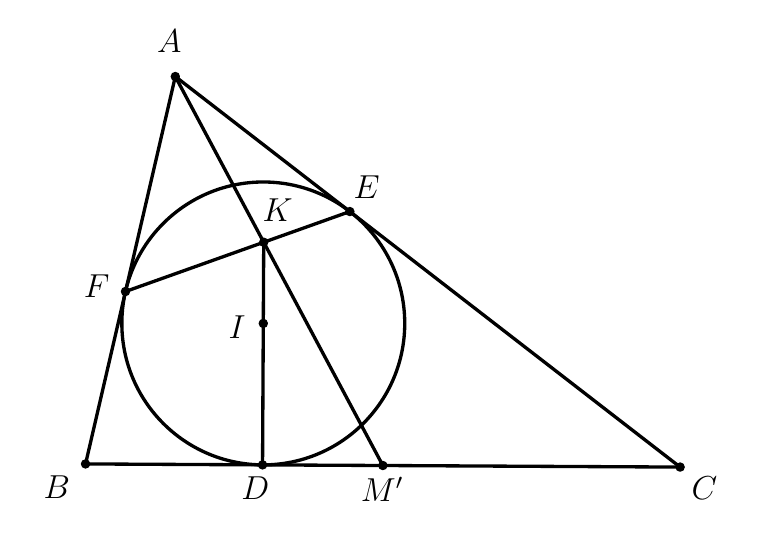
\begin{tikzpicture}[line cap=round,line join=round,>=triangle 45,x=1.0cm,y=1.0cm]
		\clip(2.1250439036274402,-1.2624451953480464) rectangle (11.133656200062438,5.040508800451184);
		\draw [line width=1.2pt] (4.,4.42)-- (2.86,-0.5);
		\draw [line width=1.2pt] (10.411122449324475,-0.5399114446100867)-- (4.,4.42);
		\draw [line width=1.2pt] (2.86,-0.5)-- (10.411122449324475,-0.5399114446100867);
		\draw [line width=1.2pt] (5.117374237077359,1.2844155388661116) circle (1.7963217951918318cm);
		\draw [line width=1.2pt] (3.3674144684740055,1.6898940218351814)-- (6.216543965673974,2.7051892364049035);
		\draw [line width=1.2pt] (4.,4.42)-- (6.635561224662235,-0.5199557223050433);
		\draw [line width=1.2pt] (5.122823709706122,2.3154389835457607)-- (5.107879913962327,-0.5118811653867775);
		\begin{scriptsize}
			\draw [fill=black] (4.,4.42) circle (1.5pt);
			\draw[color=black] (3.923691751209172,4.8637186273982795) node {\large{$A$}};
			\draw [fill=black] (2.86,-0.5) circle (1.5pt);
			\draw[color=black] (2.4939973082595905,-0.793566910294689) node {\large{$B$}};
			\draw [fill=black] (10.411122449324475,-0.5399114446100867) circle (1.5pt);
			\draw[color=black] (10.71858361985127,-0.8089399688210286) node {\large{$C$}};
			\draw [fill=black] (5.117374237077359,1.2844155388661116) circle (1.5pt);
			\draw[color=black] (4.784583028684189,1.2356768151821365) node {\large{$I$}};
			\draw [fill=black] (5.107879913962327,-0.5118811653867775) circle (1.5pt);
			\draw[color=black] (5.0151789065792824,-0.8089399688210286) node {\large{$D$}};
			\draw [fill=black] (3.3674144684740055,1.6898940218351814) circle (1.5pt);
			\draw[color=black] (3,1.7583608050776824) node {\large{$F$}};
			\draw [fill=black] (6.216543965673974,2.7051892364049035) circle (1.5pt);
			\draw[color=black] (6.429500291002524,3.02) node {\large{$E$}};
			\draw [fill=black] (5.122823709706122,2.3154389835457607) circle (1.5pt);
			\draw[color=black] (5.3,2.72) node {\large{$K$}};
			\draw [fill=black] (6.635561224662235,-0.5199557223050433) circle (1.5pt);
			\draw[color=black] (6.629350051844939,-0.8243130273473682) node {\large{$M'$}};
		\end{scriptsize}
	\end{tikzpicture}
\end{center}
\textit{By letting ID cross EF at K and demonstrating that AK passes through the midpoint of BC, we may determine the relationship between segment lengths and trignometry without having to prove that these three lines are concurrent directly.}\\
\textbf{Solution.} Let $ID$ intersect $EF$ at $K$, and $AK$ intersect $BC$ at $M'$, we will prove that $M'$ is the midpoint of $BC$.\\
We have: $\dfrac{KF}{KE}=\dfrac{AF}{AE}.\dfrac{\sin FAK}{\sin EAK}=\dfrac{\sin FAK}{\sin EAK}=\dfrac{\sin BAM'}{\sin CAM'}=\dfrac{AC}{AB}.\dfrac{BM'}{CM'}$\\\\
On the other hand: $\dfrac{KF}{KE}=\dfrac{IE}{IF}.\dfrac{\sin FIK}{\sin EIK}=\dfrac{\sin FIK}{\sin EIK}=\dfrac{\sin ABC}{\sin ACB}=\dfrac{AC}{AB}$\\\\
So we have: $\dfrac{AC}{AB}.\dfrac{BM'}{CM'}=\dfrac{AC}{AB}\implies M'B=M'C\implies M'$ is the midpoint of $BC$ $\square$
\newpage
\begin{mybox}
\textbf{Example 2.} Given $\triangle{ABC}$ inscribed in $(O)$, $(I)$ be the incircle. The incircle touch $BC, CA,AB$ at $D,E,F$ , respectively. $H$ is a point on $EF$ such that: $DH$ is perpendicular to $EF$. The line $AH$ intersects $(O)$ the second time at $G$.\\Prove that: $GD$ is the angle bisector of $\angle{BGC}$. 
\end{mybox}
\begin{center}

	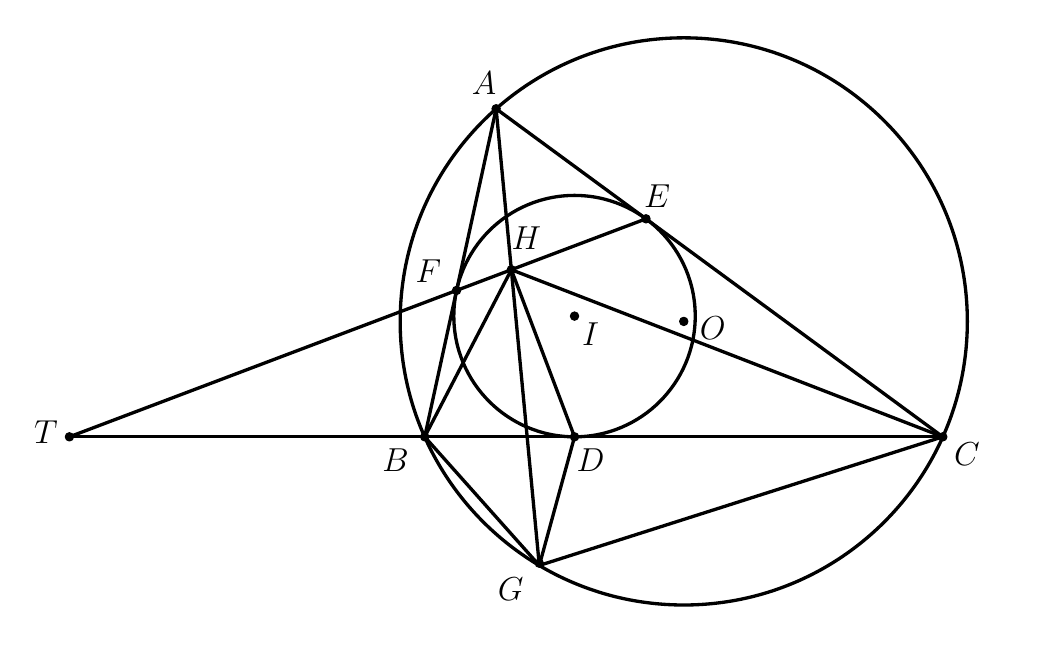
\begin{tikzpicture}[line cap=round,line join=round,>=triangle 45,x=1.0cm,y=1.0cm]
		\clip(-1.8258321376418303,-2.9996008088244177) rectangle (10.733956678377613,4.671555395819035);
		\draw [line width=1.2pt] (4.12354151205159,3.641560474554283)-- (3.2165310589975538,-0.5245383860837444);
		\draw [line width=1.2pt] (9.796200108270897,-0.5245383860837444)-- (4.12354151205159,3.641560474554283);
		\draw [line width=1.2pt] (3.2165310589975538,-0.5245383860837444)-- (9.796200108270897,-0.5245383860837444);
		\draw [line width=1.2pt] (5.119139573900037,1.0084175624967595) circle (1.5329559485805038cm);
		\draw [line width=1.2pt] (3.621271093087011,1.3345217704966434)-- (6.026544755160847,2.2439618867965363);
		\draw [line width=1.2pt] (6.506365583634225,0.9410076177095509) circle (3.601504725628705cm);
		\draw [line width=1.2pt] (-1.2955434950206797,-0.5245383860837444)-- (3.621271093087011,1.3345217704966434);
		\draw [line width=1.2pt] (-1.2955434950206797,-0.5245383860837444)-- (3.2165310589975538,-0.5245383860837444);
		\draw [line width=1.2pt] (4.316791508454673,1.5974998163692045)-- (5.1191395739000365,-0.5245383860837443);
		\draw [line width=1.2pt] (4.12354151205159,3.641560474554283)-- (4.671869312353901,-2.1582599924500623);
		\draw [line width=1.2pt] (4.671869312353901,-2.1582599924500623)-- (3.2165310589975538,-0.5245383860837444);
		\draw [line width=1.2pt] (5.1191395739000365,-0.5245383860837443)-- (4.671869312353901,-2.1582599924500623);
		\draw [line width=1.2pt] (4.671869312353901,-2.1582599924500623)-- (9.796200108270897,-0.5245383860837444);
		\draw [line width=1.2pt] (3.2165310589975538,-0.5245383860837444)-- (4.316791508454673,1.5974998163692045);
		\draw [line width=1.2pt] (4.316791508454673,1.5974998163692045)-- (9.796200108270897,-0.5245383860837444);
		\begin{scriptsize}
			\draw [fill=black] (4.12354151205159,3.641560474554283) circle (1.5pt);
			\draw[color=black] (3.9698109267881936,3.9720812328705843) node {\large{$A$}};
			\draw [fill=black] (3.2165310589975538,-0.5245383860837444) circle (1.5pt);
			\draw[color=black] (2.847577654365404,-0.8243130273473663) node {\large{$B$}};
			\draw [fill=black] (9.796200108270897,-0.5245383860837444) circle (1.5pt);
			\draw[color=black] (10.10366127879769,-0.7474477347156684) node {\large{$C$}};
			\draw [fill=black] (5.119139573900037,1.0084175624967595) circle (1.5pt);
			\draw[color=black] (5.322640077106078,0.7744850593919504) node {\large{$I$}};
			\draw [fill=black] (5.1191395739000365,-0.5245383860837443) circle (1.5pt);
			\draw[color=black] (5.322640077106078,-0.8243130273473663) node {\large{$D$}};
			\draw [fill=black] (3.621271093087011,1.3345217704966434) circle (1.5pt);
			\draw[color=black] (3.2626502345765727,1.5738841027616088) node {\large{$F$}};
			\draw [fill=black] (6.026544755160847,2.2439618867965363) circle (1.5pt);
			\draw[color=black] (6.168158296054755,2.5270137313946632) node {\large{$E$}};
			\draw [fill=black] (-1.2955434950206797,-0.5245383860837444) circle (1.5pt);
			\draw[color=black] (-1.5952362597467367,-0.4707326812415559) node {\large{$T$}};
			\draw [fill=black] (4.316791508454673,1.5974998163692045) circle (1.5pt);
			\draw[color=black] (4.50786797521008,2.0043297414991175) node {\large{$H$}};
			\draw [fill=black] (4.671869312353901,-2.13) circle (1.5pt);
			\draw[color=black] (4.3080182143676655,-2.4538572311393625) node {\large{$G$}};
			\draw [fill=black] (6.506365583634225,0.9410076177095509) circle (1.5pt);
			\draw[color=black] (6.875318988266376,0.8513503520236484) node {\large{$O$}};
		\end{scriptsize}
	\end{tikzpicture}

\end{center}
\textit{So we need to prove that $\dfrac{GB}{GC}=\dfrac{DB}{DC}$, and let's think, $\dfrac{GB}{GC}$ can be expressed in the form of $\dfrac{\sin BAG}{\sin CAG}$, and of course $\dfrac{DB}{DC}$ is too simple for us.}\\
\textbf{Solution.} Let $EF$ intersect $BC$ at $T$.\\
We have: $(TD,BC)=-1$, but $HD\perp HT$\\
$\implies HD$ is the internal bisector of $\angle{BHC}$\\$\implies \dfrac{DB}{DC}=\dfrac{HB}{HC}.$\\We also have a common properties: $\triangle{BHF}\sim \triangle{CHE},$ so by \textbf{Example 1}:$$\dfrac{DB}{DC}=\dfrac{HB}{HC}=\dfrac{HF}{HE}=\dfrac{\sin FAH}{\sin EAH}=\dfrac{\sin BAG}{\sin CAG}=\dfrac{\sin BCG}{\sin CBG}=\dfrac{GB}{GC}$$And then we are done.\\
\textbf{Remark.} To prove that $\triangle{BHF}\sim \triangle{CHE},$ we choose points $M,N$ on $EF$ such that $BM,CN$ are both perpendicular to $EF$, then we need $\triangle{BFM}\sim \triangle{CEN}$\\Then from $\dfrac{BF}{CE}=\dfrac{BM}{CN}=\dfrac{BD}{CD}=\dfrac{BH}{CH}, \triangle{BHF}\sim \triangle{CHE}$ is easily established by $S-A-S$ $\square$
\newpage
\begin{mybox}
\textbf{Example 3.} Let $I$ be the incenter of $\triangle{ABC}$. $P$ is the midpoint of arc $BC$ that does not contain $A$. $P'$ is the reflection point of $P$ through $BC$. $H$ is the orthocenter of $\triangle{BIC}$.\\Prove that: $AH, IP', BC$ are concurrent.
\end{mybox}

\begin{center}
	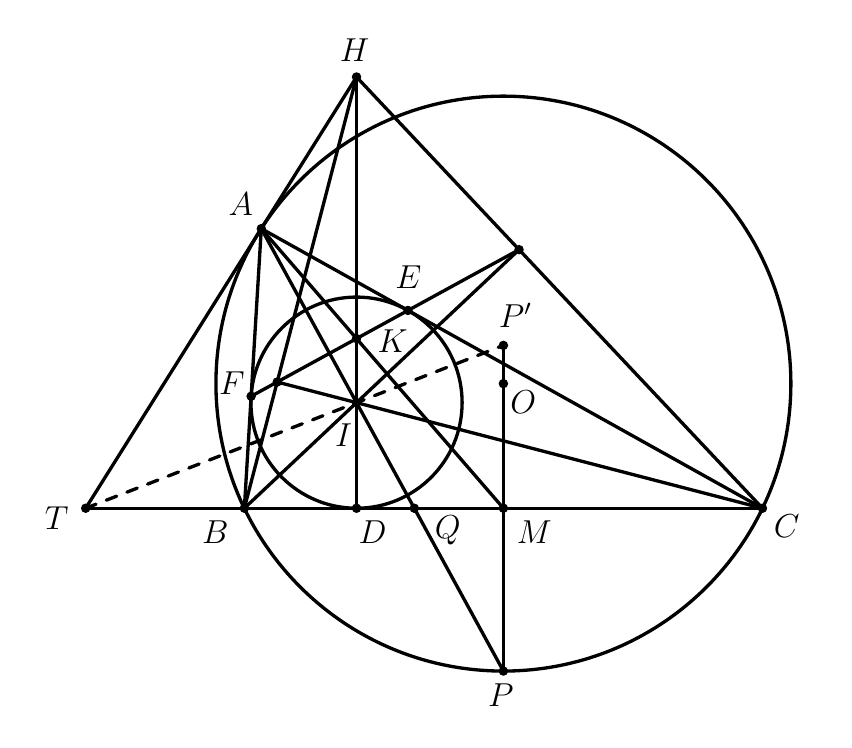
\begin{tikzpicture}[line cap=round,line join=round,>=triangle 45,x=1.0cm,y=1.0cm]
		\clip(0.46475358278276846,-3.2148236281931717) rectangle (10.580226093114216,5.578565848873071);
		\draw [line width=1.2pt] (3.4317538783663086,3.0266381335006978)-- (3.2165310589975538,-0.5245383860837444);
		\draw [line width=1.2pt] (9.796200108270897,-0.5245383860837444)-- (3.4317538783663086,3.0266381335006978);
		\draw [line width=1.2pt] (3.2165310589975538,-0.5245383860837444)-- (9.796200108270897,-0.5245383860837444);
		\draw [line width=1.2pt] (4.641140234304609,0.8163448031923608) circle (1.3408831892761053cm);
		\draw [line width=1.2pt] (3.302712877106842,0.8974616127194985)-- (5.294490861922364,1.9872848890527548);
		\draw [line width=1.2pt] (6.506365583634225,1.0581878667416702) circle (3.6507579474506624cm);
		\draw [line width=1.2pt] (1.2016099365329675,-0.5245383860837484)-- (3.2165310589975538,-0.5245383860837444);
		\draw [line width=1.2pt] (4.641140234304611,4.952408192442859)-- (1.2016099365329675,-0.5245383860837484);
		\draw [line width=1.2pt,dash pattern=on 4pt off 4pt] (1.2016099365329675,-0.5245383860837484)-- (6.506365583634225,1.5434933085415037);
		\draw [line width=1.2pt] (6.506365583634225,1.5434933085415037)-- (6.506365583634225,-2.592570080708992);
		\draw [line width=1.2pt] (4.641140234304611,4.952408192442859)-- (3.2165310589975538,-0.5245383860837444);
		\draw [line width=1.2pt] (4.641140234304611,4.952408192442859)-- (9.796200108270897,-0.5245383860837444);
		\draw [line width=1.2pt] (6.705384321914347,2.7592707955382316)-- (3.2165310589975538,-0.5245383860837444);
		\draw [line width=1.2pt] (5.294490861922364,1.9872848890527548)-- (6.705384321914347,2.7592707955382316);
		\draw [line width=1.2pt] (3.6334836267620436,1.078446473910153)-- (9.796200108270897,-0.5245383860837444);
		\draw [line width=1.2pt] (4.641140234304609,0.8163448031923608)-- (4.6411402343046095,-0.5245383860837444);
		\draw [line width=1.2pt] (3.4317538783663086,3.0266381335006978)-- (6.506365583634225,-2.592570080708992);
		\draw [line width=1.2pt] (4.641140234304611,4.952408192442859)-- (4.641140234304609,0.8163448031923608);
		\draw [line width=1.2pt] (3.4317538783663086,3.0266381335006978)-- (6.506365583634226,-0.5245383860837444);
		\begin{scriptsize}
			\draw [fill=black] (3.4317538783663086,3.0266381335006978) circle (1.5pt);
			\draw[color=black] (3.1704118834185357,3.341785833290661) node {\large{$A$}};
			\draw [fill=black] (3.2165310589975538,-0.5245383860837444) circle (1.5pt);
			\draw[color=black] (2.8475776543654043,-0.8243130273473663) node {\large{$B$}};
			\draw [fill=black] (9.796200108270897,-0.5245383860837444) circle (1.5pt);
			\draw[color=black] (10.10366127879769,-0.7474477347156684) node {\large{$C$}};
			\draw [fill=black] (4.641140234304609,0.8163448031923608) circle (1.5pt);
			\draw[color=black] (4.477121858157401,0.40553165475980046) node {\large{$I$}};
			\draw [fill=black] (4.6411402343046095,-0.5245383860837444) circle (1.5pt);
			\draw[color=black] (4.846075262789551,-0.8243130273473663) node {\large{$D$}};
			\draw [fill=black] (3.302712877106842,0.8974616127194985) circle (1.5pt);
			\draw[color=black] (3.06,1.0665731713924027) node {\large{$F$}};
			\draw [fill=black] (5.294490861922364,1.9872848890527548) circle (1.5pt);
			\draw[color=black] (5.3,2.4040292631839466) node {\large{$E$}};
			\draw [fill=black] (6.506365583634225,1.0581878667416702) circle (1.5pt);
			\draw[color=black] (6.76,0.8206042349709692) node {\large{$O$}};
			\draw [fill=black] (6.506365583634225,-2.592570080708992) circle (1.5pt);
			\draw[color=black] (6.475619466581547,-2.8996759284032105) node {\large{$P$}};
			\draw [fill=black] (6.506365583634225,1.5434933085415037) circle (1.5pt);
			\draw[color=black] (6.6600961688976215,1.9274644488674193) node {\large{$P'$}};
			\draw [fill=black] (6.705384321914347,2.7592707955382316) circle (1.5pt);
			\draw [fill=black] (3.6334836267620436,1.078446473910153) circle (1.5pt);
			\draw [fill=black] (4.641140234304611,4.952408192442859) circle (1.5pt);
			\draw[color=black] (4.615479384894457,5.294164266135789) node {\large{$H$}};
			\draw [fill=black] (1.2016099365329675,-0.5245383860837484) circle (1.5pt);
			\draw[color=black] (0.8337069874149186,-0.6552093835576309) node {\large{$T$}};
			\draw [fill=black] (6.506365583634226,-0.5245383860837444) circle (1.5pt);
			\draw[color=black] (6.9,-0.8243130273473663) node {\large{$M$}};
			\draw [fill=black] (5.374819249565145,-0.5245383860837444) circle (1.5pt);
			\draw[color=black] (5.8,-0.8) node {\large{$Q$}};
			\draw [fill=black] (4.641140234304609,1.6297968923919617) circle (1.5pt);
			\draw[color=black] (5.1,1.6) node {\large{$K$}};
		\end{scriptsize}
	\end{tikzpicture}
\end{center}
\textit{Like \textbf{Example 2}, we just let $AH$ intersects $BC$ at $T$, and prove that $T,I,P'$ are collinear, but notice that $ID\parallel P'M$, consequently, this brings to mind Property \textbf{2} as from the beginning..}\\
\textbf{Solution.} Let $AH$ intersects $BC$ at $T$, $ID$ intersects $EF$ at $K$, and $AI$ intersects $BC$ at $Q$.\\
We need to prove that: $\dfrac{TD}{TM}=\dfrac{ID}{P'M}$, but $\dfrac{ID}{P'M}=\dfrac{QD}{QM}$.\\
This means we want to have:$\dfrac{TD}{TM}=\dfrac{QD}{QM}$, or $(TQ,DM)=-1$.
By the result of \textbf{Example 1}, we have: $A,K,M$ are collinear.\\
Take $A$ as the projection center: $A(TQ,DM)=A(HI,DK)=-1$ (Since $BI$ and $CH$ intersect on $EF$, and $CI$ and $BH$ intersect on $EF$).\\
In conclusion: We have $(TQ,DM)=-1$, and that results in the desired goal.\\
To demonstrate the strength of this tool, let's try some more challenging problems:
\newpage
\begin{mybox}
\textbf{Example 4.} Given an acute triangle $ABC$ inscribed in $(O)$ with $H$ be the orthocenter. $AH, BH, CH$ cuts $BC, CA, AB$ at $D, E, F$ and $I, M, N$ are the midpoints of $BC, HB, HC$. $BH, CH$ cuts $(O)$ at $L,K(L \ne B, K \ne C)$; $KL$ cuts $MN$ at $G$.
\begin{enumerate}
 \item We choose a point $T$ on $EF$ such that $AT\perp IH$. Prove that: $GT \perp OH$.
 \item $DE, DF$ cut $MN$ at $P, Q$, respectively. Let $S$ be the intersection point of $BQ,CP$.\\Prove that: $HS$ bisects $EF$.
\end{enumerate}
\end{mybox}

\begin{center}

		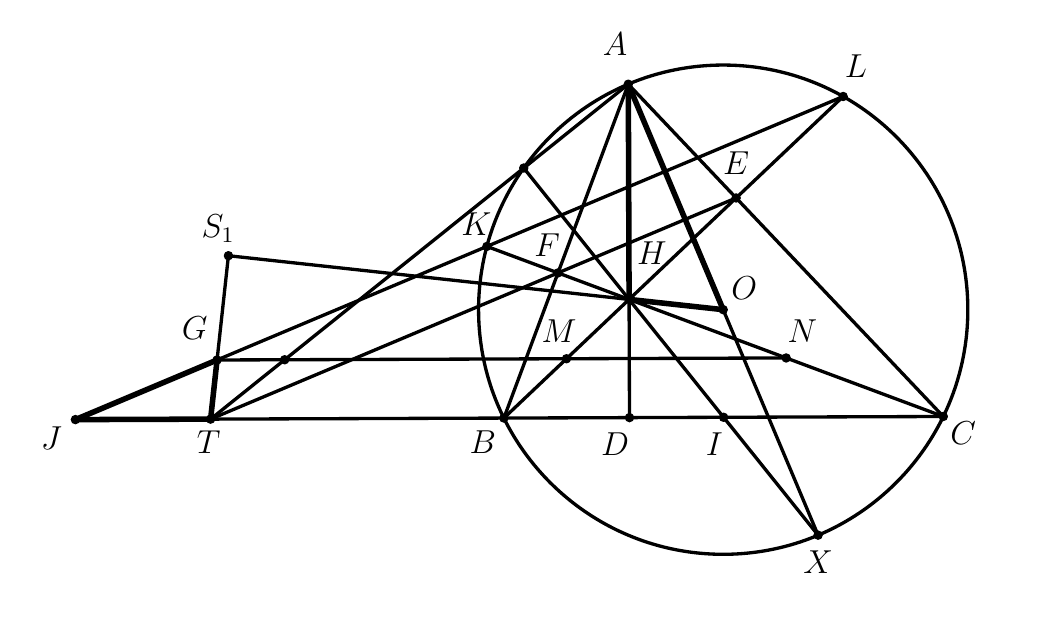
\begin{tikzpicture}[line cap=round,line join=round,>=triangle 45,x=1.0cm,y=1.0cm]
			\clip(-1.348,-3.422) rectangle (11.452,3.958);
			\draw [line width=1.2pt] (6.28,3.24)-- (4.7,-1.);
			\draw [line width=1.2pt] (4.7,-1.)-- (10.28,-0.98);
			\draw [line width=1.2pt] (6.28,3.24)-- (10.28,-0.98);
			\draw [line width=1.2pt] (7.485101999356686,0.3765421794850091) circle (3.106712332792005cm);
			\draw [line width=1.2pt] (7.649221850191077,1.7954709480484137)-- (4.7,-1.);
			\draw [line width=1.2pt] (1.0570476021859856,-0.2624484533146056)-- (9.008647699095524,3.0840262550668474);
			\draw [line width=1.2pt] (1.0570476021859856,-0.2624484533146056)-- (8.284898000643315,-0.23654217948500939);
			\draw [line width=1.2pt] (4.484033831672243,1.1798175815938332)-- (10.28,-0.98);
			\draw [line width=1.2pt] (7.649221850191077,1.7954709480484137)-- (9.008647699095524,3.0840262550668474);
			\draw [line width=2.pt] (-0.7418030734135962,-1.0195046705140272)-- (1.0570476021859856,-0.2624484533146056);
			\draw [line width=1.2pt] (4.952101751220348,2.175311553713733)-- (8.690203998713372,-2.486915641029981);
			\draw [line width=1.2pt] (6.28,3.24)-- (0.9751457883369482,-1.0133507319414445);
			\draw [line width=1.2pt] (0.9751457883369482,-1.0133507319414445)-- (7.649221850191077,1.7954709480484137);
			\draw [line width=2.pt] (-0.7418030734135962,-1.0195046705140272)-- (0.9751457883369482,-1.0133507319414445);
			\draw [line width=1.2pt] (0.9751457883369482,-1.0133507319414445)-- (4.7,-1.);
			\draw [line width=1.2pt] (1.2014961649922695,1.0619026185131568)-- (1.0570476021859856,-0.2624484533146056);
			\draw [line width=2.pt] (1.0570476021859856,-0.2624484533146056)-- (0.9751457883369482,-1.0133507319414445);
			\draw [line width=2.pt] (6.28,3.24)-- (6.28979600128663,0.5069156410299812);
			\draw [line width=1.2pt] (6.28979600128663,0.5069156410299812)-- (6.295176639860229,-0.9942825210040853);
			\draw [line width=2.pt] (6.28,3.24)-- (7.485101999356686,0.3765421794850091);
			\draw [line width=2.pt] (6.28979600128663,0.5069156410299812)-- (7.485101999356686,0.3765421794850091);
			\draw [line width=1.2pt] (6.28979600128663,0.5069156410299812)-- (1.2014961649922695,1.0619026185131568);
			\draw [line width=1.2pt] (7.485101999356686,0.3765421794850091)-- (8.690203998713372,-2.486915641029981);
			\begin{scriptsize}
				\draw [fill=black] (6.28,3.24) circle (1.5pt);
				\draw[color=black] (6.112,3.748) node {\large{$A$}};
				\draw [fill=black] (4.7,-1.) circle (1.5pt);
				\draw[color=black] (4.432,-1.3) node {\large{$B$}};
				\draw [fill=black] (10.28,-0.98) circle (1.5pt);
				\draw[color=black] (10.532,-1.192) node {\large{$C$}};
				\draw [fill=black] (6.295176639860229,-0.9942825210040853) circle (1.5pt);
				\draw[color=black] (6.112,-1.332) node {\large{$D$}};
				\draw [fill=black] (7.649221850191077,1.7954709480484137) circle (1.5pt);
				\draw[color=black] (7.65,2.24) node {\large{$E$}};
				\draw [fill=black] (5.386914916479437,0.8433666113119074) circle (1.5pt);
				\draw[color=black] (5.25,1.2) node {\large{$F$}};
				\draw [fill=black] (6.28979600128663,0.5069156410299812) circle (1.5pt);
				\draw[color=black] (6.58,1.1) node {\large{$H$}};
				\draw [fill=black] (7.49,-0.99) circle (1.5pt);
				\draw[color=black] (7.372,-1.332) node {\large{$I$}};
				\draw [fill=black] (5.494898000643316,-0.2465421794850094) circle (1.5pt);
				\draw[color=black] (5.4,0.108) node {\large{$M$}};
				\draw [fill=black] (8.284898000643315,-0.23654217948500939) circle (1.5pt);
				\draw[color=black] (8.492,0.108) node {\large{$N$}};
				\draw [fill=black] (4.484033831672243,1.1798175815938332) circle (1.5pt);
				\draw[color=black] (4.35,1.468) node {\large{$K$}};
				\draw [fill=black] (9.008647699095524,3.0840262550668474) circle (1.5pt);
				\draw[color=black] (9.172,3.47) node {\large{$L$}};
				\draw [fill=black] (1.0570476021859856,-0.2624484533146056) circle (1.5pt);
				\draw[color=black] (0.772,0.148) node {\large{$G$}};
				\draw [fill=black] (-0.7418030734135962,-1.0195046705140272) circle (1.5pt);
				\draw[color=black] (-1.048,-1.252) node {\large{$J$}};
				\draw [fill=black] (7.485101999356686,0.3765421794850091) circle (1.5pt);
				\draw[color=black] (7.752,0.648) node {\large{$O$}};
				\draw [fill=black] (8.690203998713372,-2.486915641029981) circle (1.5pt);
				\draw[color=black] (8.692,-2.832) node {\large{$X$}};
				\draw [fill=black] (4.952101751220348,2.175311553713733) circle (1.5pt);
				\draw [fill=black] (1.9155220330612626,-0.2593714840283143) circle (1.5pt);
				\draw [fill=black] (0.9751457883369482,-1.0133507319414445) circle (1.5pt);
				\draw[color=black] (0.952,-1.312) node {\large{$T$}};
				\draw [fill=black] (1.2014961649922695,1.0619026185131568) circle (1.5pt);
				\draw[color=black] (1.072,1.4) node {\large{$S_1$}};
			\end{scriptsize}
		\end{tikzpicture}

\end{center}

\textbf{Solution.}\\
1) Let $S_1$ be the intersection point of $GT$ and $HO$, according to the hypothesis, $AT$ goes through the intersection point of $(AH)$ and $(O)$, and $T$ lies on $EF$\\So by the Radical axis theorem for $(AH), (O), (EFBC)$: $T \in BC$.\\
We have: $\dfrac{JG}{JK}=\dfrac{CN}{CK};\dfrac{JT}{JC}=\dfrac{KF}{KC}$(By Thales therem)\\\\
$\implies \dfrac{JG}{JT}.\dfrac{JC}{JK}=\dfrac{CN}{CK}.\dfrac{CK}{KF}=\dfrac{CN}{KF}$\\\\
$\implies \dfrac{JG}{JT}=\dfrac{CN}{KF}.\dfrac{JK}{JC}=\dfrac{CN}{KF}.\dfrac{KB}{LC}$ (Since $\triangle{JKB}\sim \triangle{JCL}$)=$\dfrac{CN}{KF}.\dfrac{KH}{LH}=\dfrac{CH}{KH}.\dfrac{KH}{LH}=\dfrac{CH}{LH}$\\
Now we will prove that: $\triangle{JGT} \sim \triangle{AHO}$\\ But we already have: $\angle{HAO}=\angle{TJG}$ (Because $AO\perp JL$ and $AD\perp JD$), so it seems sense to prove that: $\dfrac{AH}{AO}=\dfrac{JG}{JT}$, or $\dfrac{AL}{AO}=\dfrac{CH}{LH}$ ($AL=AH$), and it's true since $\triangle{AOL}\sim \triangle{HCL}$.\\
So: $\triangle{JGT} \sim \triangle{AHO} \implies \angle{AHO}=\angle{JTG}\implies TS_1HD$ is a cyclic quadrilateral $\square$
\newpage
2) This appears to be an impossible question to answer using trigonometric ratio, right?\\But let's give it a try, though.
\begin{center}

	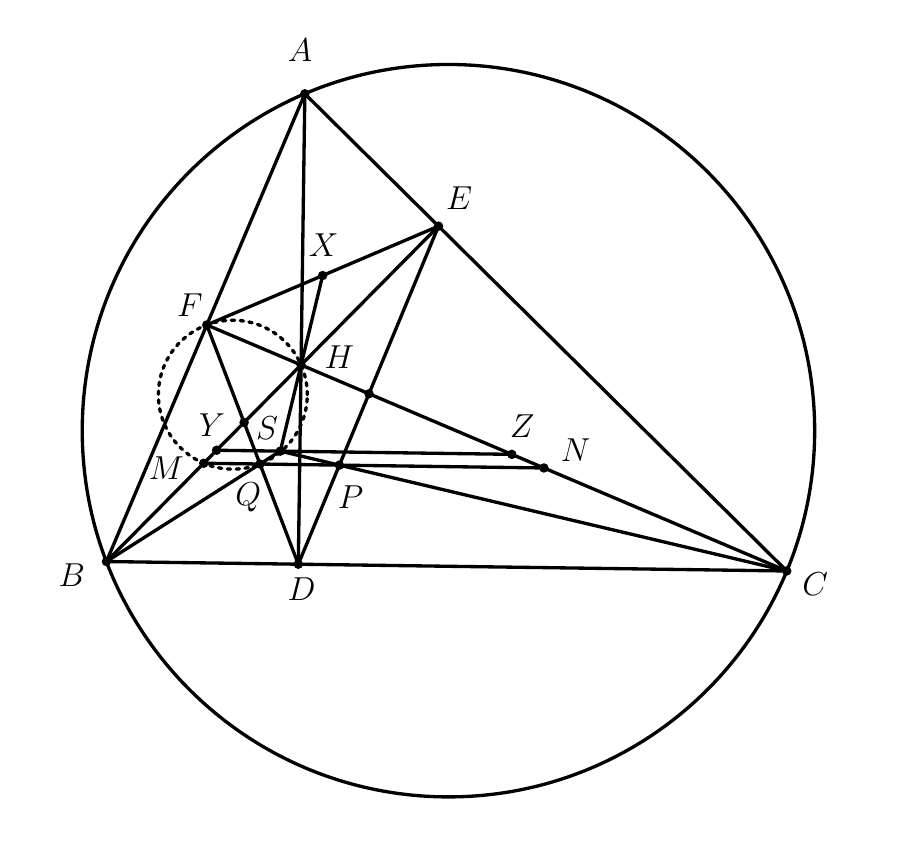
\begin{tikzpicture}[line cap=round,line join=round,>=triangle 45,x=1.0cm,y=1.0cm]
		\clip(-0.36,-4.94) rectangle (10.44,5.26);
		\draw [line width=1.2pt] (3.16,4.42)-- (0.64,-1.52);
		\draw [line width=1.2pt] (0.64,-1.52)-- (9.28,-1.64);
		\draw [line width=1.2pt] (9.28,-1.64)-- (3.16,4.42);
		\draw [line width=1.2pt] (4.983912133891212,0.14167364016736406) circle (4.650885067747253cm);
		\draw [line width=1.2pt] (1.914708171206226,1.4846692607003893)-- (3.077029893924783,-1.5538476374156223);
		\draw [line width=1.2pt] (4.857442368357194,2.739199223489443)-- (3.077029893924783,-1.5538476374156223);
		\draw [line width=1.2pt] (1.876087866108787,-0.2716736401673641)-- (6.196087866108787,-0.33167364016736406);
		\draw [line width=1.2pt] (2.8480927936165132,-0.11794014912517795)-- (0.64,-1.52);
		\draw [line width=1.2pt] (2.8480927936165132,-0.11794014912517795)-- (9.28,-1.64);
		\draw [line width=1.2pt] (1.914708171206226,1.4846692607003893)-- (4.857442368357194,2.739199223489443);
		\draw [line width=1.2pt] (3.16,4.42)-- (3.077029893924783,-1.5538476374156223);
		\draw [line width=1.2pt] (0.64,-1.52)-- (4.857442368357194,2.739199223489443);
		\draw [line width=1.2pt] (1.914708171206226,1.4846692607003893)-- (9.28,-1.64);
		\draw [line width=1.2pt] (3.3860752697817107,2.1119342420949168)-- (2.8480927936165132,-0.11794014912517795);
		\draw [line width=1.2pt] (2.0394354073494934,-0.10670879653813602)-- (5.788552545776491,-0.1587798679051776);
		\draw [line width=1.2pt,dotted] (2.245380573694439,0.5988020277131005) circle (0.9455712518091278cm);
		\begin{scriptsize}
			\draw [fill=black] (3.16,4.42) circle (1.5pt);
			\draw[color=black] (3.1,4.97) node {\large{$A$}};
			\draw [fill=black] (0.64,-1.52) circle (1.5pt);
			\draw[color=black] (0.2,-1.69) node {\large{$B$}};
			\draw [fill=black] (9.28,-1.64) circle (1.5pt);
			\draw[color=black] (9.64,-1.81) node {\large{$C$}};
			\draw [fill=black] (3.077029893924783,-1.5538476374156223) circle (1.5pt);
			\draw[color=black] (3.12,-1.87) node {\large{$D$}};
			\draw [fill=black] (4.857442368357194,2.739199223489443) circle (1.5pt);
			\draw[color=black] (5.12,3.09) node {\large{$E$}};
			\draw [fill=black] (1.914708171206226,1.4846692607003893) circle (1.5pt);
			\draw[color=black] (1.7,1.73) node {\large{$F$}};
			\draw [fill=black] (3.112175732217574,0.9766527196652718) circle (1.5pt);
			\draw[color=black] (3.6,1.08) node {\large{$H$}};
			\draw [fill=black] (2.388577478326686,0.24589012662694976) circle (1.5pt);
			\draw [fill=black] (3.9747212209395353,0.6107243305105007) circle (1.5pt);
			\draw [fill=black] (1.876087866108787,-0.2716736401673641) circle (1.5pt);
			\draw[color=black] (1.4,-0.33) node {\large{$M$}};
			\draw [fill=black] (6.196087866108787,-0.33167364016736406) circle (1.5pt);
			\draw[color=black] (6.6,-0.11) node {\large{$N$}};
			\draw [fill=black] (2.590355618485498,-0.2815940256170406) circle (1.5pt);
			\draw[color=black] (2.44,-0.7) node {\large{$Q$}};
			\draw [fill=black] (3.5988500076568593,-0.29560089213330953) circle (1.5pt);
			\draw[color=black] (3.74,-0.7) node {\large{$P$}};
			\draw [fill=black] (2.8480927936165132,-0.11794014912517795) circle (1.5pt);
			\draw[color=black] (2.68,0.17) node {\large{$S$}};
			\draw [fill=black] (3.3860752697817107,2.1119342420949168) circle (1.5pt);
			\draw[color=black] (3.4,2.5) node {\large{$X$}};
			\draw [fill=black] (5.788552545776491,-0.1587798679051776) circle (1.5pt);
			\draw[color=black] (5.92,0.2) node {\large{$Z$}};
			\draw [fill=black] (2.0394354073494934,-0.10670879653813602) circle (1.5pt);
			\draw[color=black] (1.98,0.21) node {\large{$Y$}};
		\end{scriptsize}
	\end{tikzpicture}
\end{center}
\textit{To support your ideas, you may occasionally need to construct objects like parallel and perpendicular lines. Keep in mind that ratios are not always obvious for you to transform.}\\
\textbf{Solution.}\\
2) Let $X$ be the intersection point of $HS$ and $EF$. We will prove that $X$ is the midpoint of $EF$.\\
We have: $\dfrac{XE}{XF}=\dfrac{HE}{HF}.\dfrac{\sin {EHX}}{\sin {FHX}}=\dfrac{HE}{HF}.\dfrac{\sin {BHS}}{\sin {CHS}}$, and $\dfrac{SY}{SZ}=\dfrac{\sin BHS}{\sin CHS}.\dfrac{HY}{HZ}$\\\\
$\implies \dfrac{XE}{XF}=\dfrac{SY}{SZ}.\dfrac{HE}{HF}.\dfrac{HZ}{HY}=\dfrac{SY}{SZ}.\dfrac{HE}{HF}.\dfrac{HC}{HB}$\\
So all we need to do is to prove that: $$\dfrac{SY}{SZ}.\dfrac{HE}{HF}.\dfrac{HC}{HB}=1$$
Indeed, $\dfrac{SY}{MQ}=\dfrac{BS}{BQ};\dfrac{SZ}{NP}=\dfrac{CS}{CP}$ (By Thales Theorem) $\implies \dfrac{{SY}}{{SZ}}.\dfrac{{NP}}{{MQ}} = \dfrac{{BS}}{{BQ}}.\dfrac{{CP}}{{CS}}=1$ (Thales theorem again) $\implies \dfrac{{SY}}{{SZ}}=\dfrac{{MQ}}{{NP}}$\\\\
Similar to the "trick" above: $\dfrac{{MQ}}{{MH}} = \dfrac{{\sin MHQ}}{{\sin MQH}};\dfrac{{NH}}{{NP}} = \dfrac{{\sin NPH}}{{\sin NHP}}$\\$\implies \dfrac{{MQ}}{{NP}}.\dfrac{{NH}}{{MH}} = \dfrac{{\sin MHQ}}{{\sin MQH}}.\dfrac{{\sin NPH}}{{\sin NHP}}$\\
We easily have: $\triangle{HPQ}$ is isosceles $\implies \angle{MQH}=\angle{NPH}$\\\\
$\implies \dfrac{{MQ}}{{NP}}.\dfrac{{NH}}{{MH}} = \dfrac{{\sin MHQ}}{{\sin NHP}}$, but notice that: $\angle{MHQ}=\angle{MDF}=\angle{BDF}-\angle{MDB}=\angle{BHF}-\angle{MBD}=\angle{BHF}-\angle{HFE}=\angle{HEF}$
\\And similarly: $\angle{NHP}=\angle{HFE}$\\\\
So $\dfrac{{MQ}}{{NP}}.\dfrac{{NH}}{{MH}} = \dfrac{{\sin HEF}}{{\sin HFE}}\implies \dfrac{SY}{SZ}= \dfrac{{MQ}}{{NP}}=\dfrac{{MH}}{{NH}} .\dfrac{{\sin HEF}}{{\sin HFE}}=\dfrac{HB}{HC}.\dfrac{{\sin HEF}}{{\sin HFE}}$\\
So the thing that we need for this problem is deduced to:$$\dfrac{HB}{HC}.\dfrac{{\sin HEF}}{{\sin HFE}}.\dfrac{HE}{HF}.\dfrac{HC}{HB}=1$$
which is trivial by the Law of Sines.
\\\\\\\\\\\\\\\\\\\\\\\\\\\\\\\\\\\\
\textbf{\underline{\Large{Remark on section 2.}}}\\
\textbf{$-$ The skill you must master is computing the difficult-to-bash terms using the way in which they can cancel one another out while multiplying.\\$-$ Sound ethereal? Try to solve more problems using ratio transforming, and after each problem you solve, read YOUR solution again and figure out how you linked these ratios!}





\newpage
\section{Training problems}
\textbf{1.(MEMO 2016)} Let $ABC$ be an acute triangle for which $AB \neq AC$, and let $O$ be its circumcenter. Line $AO$ meets the circumcircle of $ABC$ again in $D$, and the line $BC$ in $E$. The circumcircle of $CDE$ meets the line $CA$ again in $P$. The lines $PE$ and $AB$ intersect in $Q$. Line passing through $O$ parallel to the line $PE$ intersects the $A$-altitude of $ABC$ at $F$.\\
Prove that: $FP = FQ$.\\

\textbf{2.(ISL 2015)} Let $ABC$ be an acute triangle with orthocenter $H$. Let $G$ be the point such that the quadrilateral $ABGH$ is a parallelogram. Let $I$ be the point on the line $GH$ such that $AC$ bisects $HI$. Suppose that the line $AC$ intersects the circumcircle of the triangle $GCI$ at $C$ and $J$.\\Prove that: $IJ = AH$.\\

\textbf{3.(CHKMO 2021)} Let $ABCD$ be a cyclic quadrilateral inscribed in $\Gamma$ such that $AB=AD$. Let $E$ be a point on the segment $CD$ such that $BC=DE$. The line $AE$ intersect $\Gamma$ again at $F$. The chords $AC$ and $BF$ meet at $M$. Let $P$ be the symmetric point of $C$ about $M$.\\
Prove that: $PE$ and $BF$ are parallel.\\

\textbf{4.(Adapted from VIASM Summer Camp 2022)} Given an acute not isosceles triangle $ABC$ inscribed in $(O)$. Choose points $M,N,P$ on $AB,BC,CA$ such that $AMNP$ is a parallelogram. The segment $CM$ cuts $NP$ at $E$, the segment $BP$ cuts $NM$ at $F$. The segment $BE$ cuts $CF$ at $D$.\\
Prove that: $A,D,N$ are collinear.\\

\textbf{5.(Iranian TST 2020)} Given a triangle $ABC$ with circumcircle $\Gamma$. Points $E$ and $F$ are the foot of angle bisectors of $B$ and $C$, $I$ is incenter and $K$ is the intersection of $AI$ and $EF$. Suppose that $T$ be the midpoint of arc $BAC$. Circle $\Gamma$ intersects the $A$-median and circumcircle of $AEF$ for the second time at $X$ and $S$. Let $S'$ be the reflection of $S$ across $AI$ and $J$ be the second intersection of circumcircle of $AS'K$ and $AX$.
\\Prove that: the quadrilateral $TJIX$ is cyclic.\\

\textbf{6.(Baltic Way 2021)} Let $D$ be the foot of the $A$-altitude of an acute triangle $ABC$. The internal bisector of the angle $DAC$ intersects $BC$ at $K$. Let $L$ be the projection of $K$ onto $AC$. Let $M$ be the intersection point of $BL$ and $AD$. Let $P$ be the intersection point of $MC$ and $DL$.
\\Prove that: $PK$ is perpendicular to $AB$.\\

\textbf{7.(Vietnamese Northern Delta And Coastal Area Olympiad 2022)} Given a triangle $ABC$ inscribed in $(O)$, $AB<AC$ and the internal angle bisector of $\angle{BAC}$ intersects $BC, (O)$ at $D,E$, respectively. $M$ is the midpoint of $AD$. $BM$ intersects $(O)$ at $P$ $(P\ne B)$. $EP$ cuts $AC$ at $N$.
\begin{enumerate}
	\item Prove that: $N$ is the midpoint of $AC$
	\item Assume that $(EMN)$ cuts $BM$ at $R$ $(R\ne M)$.\\Prove that: $RA\perp RC$.
\end{enumerate}

\textbf{8.(Vietnamese HSGS Olympiad 2022)} Given a non-isosceles triangle $ABC$, $(I)$ is its incircle. $(I)$ touch $BC,CA,AB$ at $D,E,F$, respectively. The lines $IB, IC$ cuts $EF$ at $M,N$, respectively. Choose points $P,Q$ on $IC,IB$ such that $MP$ and $NQ$ are perpendicular to $BC$.
\begin{enumerate}
	\item Prove that: $BP,CQ,ID$ are concurrent at a point, let its name $T$.
	\item Let $ID$ intersects $PQ$ at $Y$, $EP$ intersects $FQ$ at $Z$.\\Prove that: $EQ, FP, AT, YZ$ are concurrent. 
\end{enumerate}  

\textbf{9.(Iranian TST 2021)} In acute scalene triangle $ABC$ the external angle bisector of $\angle BAC$ meet $BC$ at point $X$.Lines $l_b$ and $l_c$ which tangents of $B$ and $C$ with respect to $(ABC)$.The line pass through $X$ intersects $l_b$ and $l_c$ at points $Y$ and $Z$ respectively. Let $(AYB)\cap(AZC)=N$ and $l_b\cap l_c=D$.\\
Prove that: $ND$ is angle bisector of $\angle YNZ$.\\

\textbf{10.(Iranian TST 2017)} In triangle $ABC$ let $O$ and $H$ be the circumcenter and the orthocenter. The point $P$ is the reflection of $A$ with respect to $OH$. Assume that $P$ is not on the same side of $BC$ as $A$. Points $E,F$ lie on $AB,AC$ respectively such that $BE=PC \ ,  CF=PB$. Let $K$ be the intersection point of $AP,OH$.\\Prove that: $\angle EKF = 90 ^{\circ}$\\

\textbf{11.(IMO 2010)} Let $P$ be a point interior to triangle $ABC$ (with $CA \neq CB$). The lines $AP$, $BP$ and $CP$ meet again its circumcircle $\Gamma$ at $K$, $L$, respectively $M$. The tangent line at $C$ to $\Gamma$ meets the line $AB$ at $S$.\\ Prove that: if $SC = SP$, then $MK = ML$.\\

\textbf{12.(ISL 2012)} Let $ABC$ be an acute-angled triangle and let $D, E$, and $F$ be the feet of altitudes from $A, B$, $C$ to sides $BC, CA$, $AB$, respectively. Denote by $\omega_B$ and $\omega_C$ the incircles of triangles $BDF$ and $CDE$, and let these circles be tangent to segments $DF$ and $DE$ at $M$ and $N$, respectively. Let line $MN$ meet circles $\omega_B$ and $\omega_C$ again at $P \ne M$ and $Q \ne N$, respectively.\\Prove that: $MP = NQ$.\\

\textbf{13.(Sharygin 2013)} The altitudes $AA_1, BB_1, CC_1$ of an acute triangle $ABC$ concur at $H$. The perpendicular lines from $H$ to $B_1C_1, A_1C_1$ meet rays $CA, CB$ at $P, Q$ respectively.\\
Prove that: the line from $C$ perpendicular to $A_1B_1$ passes through the midpoint of $PQ$.\\

\textbf{14.(ISL 2017)} Let $ABCDE$ be a convex pentagon such that $AB=BC=CD$, $\angle{EAB}=\angle{BCD}$, and $\angle{EDC}=\angle{CBA}$.\\Prove that: the perpendicular line from $E$ to $BC$ and the lines $AC$ and $BD$ are concurrent.
\newpage
\begin{thebibliography}{widest entry}
 \bibitem[1]{cite_key1} AoPS Community: \url{https://artofproblemsolving.com/community}
 \bibitem[2]{cite_key2} l l w y s Math Blog: \url{https://llwys.blogspot.com}
 \bibitem[3]{cite_key3} Geometry problems from IMO (Shortlists), MEMO, Baltic Way, Sharygin, Iranian TST, CHKMO, Vietnamese Math Contests For High School Students, ...
\end{thebibliography}






\end{document}